\documentclass[9.5pt,a4paper]{article}

% Packages
\usepackage[utf8]{inputenc}
\usepackage[T1]{fontenc}
\usepackage[margin=2.5cm]{geometry}
\usepackage{helvet}
\renewcommand{\familydefault}{\sfdefault}
\usepackage{fancyhdr}
\usepackage{tikz}
\usetikzlibrary{shapes.geometric, arrows.meta, positioning, fit, backgrounds, calc}
\usepackage{booktabs}
\usepackage{array}
\usepackage{longtable}
\usepackage{graphicx}
\usepackage[hidelinks]{hyperref}
\usepackage{xcolor}
\usepackage{setspace}
\usepackage{pdflscape}
\usepackage{float}

% Header and footer configuration
\pagestyle{fancy}
\fancyhf{}
\fancyfoot[C]{\thepage}
\renewcommand{\headrulewidth}{0pt}
\renewcommand{\footrulewidth}{0pt}

% Landscape page style
\fancypagestyle{lscape}{%
  \fancyhf{}
  \fancyfoot{%
    \tikz[remember picture,overlay] \node[rotate=90,anchor=south] at (current page.east) {\thepage};
  }
  \renewcommand{\headrulewidth}{0pt}
  \renewcommand{\footrulewidth}{0pt}
}

% Color definitions
\definecolor{boxfill}{RGB}{245,245,245}
\definecolor{boxborder}{RGB}{200,200,200}
% Grayscale palette for methodology diagram
\definecolor{stepcolor}{RGB}{255,255,255}       % White for step boxes
\definecolor{outputcolor}{RGB}{245,245,245}     % Light gray for outputs
\definecolor{arrowcolor}{RGB}{0,0,0}            % Black for main arrows
\definecolor{reusecolor}{RGB}{120,120,120}      % Medium gray for reuse arrows
\definecolor{bordercolor}{RGB}{60,60,60}        % Dark gray for borders
\definecolor{phasebg}{RGB}{230,230,230}         % Light gray for phase labels

\begin{document}

\begin{center}
\fontsize{11}{13}\selectfont\bfseries
Tables and Diagram - Thesis (Methodology + Data)\\
\vspace{0.5em}
\fontsize{9.5}{11}\selectfont\normalfont
Coupling Remote Sensing, Morphology, and Microclimate Simulation to Analyse Urban Heat
\end{center}

\vspace{1em}

\noindent\textbf{Compilation notes:} This file is pure LaTeX and does not require Python. To compile, run:
\begin{verbatim}
pdflatex 071225_table_diagram.tex
\end{verbatim}
or alternatively:
\begin{verbatim}
xelatex 071225_table_diagram.tex
\end{verbatim}

\vspace{1em}

% TABLE 1: Data Sources
\begin{table}[p]
\centering
\fontsize{6.5}{7.5}\selectfont
\caption{Data sources (all inputs are open-access)}
\label{tab:data}
\vspace{0.3cm}
\setlength{\tabcolsep}{3pt}
\begin{tabular}{@{}p{1.3cm}p{14.7cm}@{}}
\toprule
\textbf{Step} & \textbf{Raw Data Sources} \\
\midrule
\multicolumn{2}{p{16cm}}{\textit{Abbrev.: L8/9 = Landsat~8/9; GEE = Google Earth Engine; LST = Land Surface Temperature; Ta = air temperature; DEM/DSM = Digital Elevation/Surface Model; GOB = Google Open Buildings; OSM = OpenStreetMap; INEGI = Instituto Nacional de Estadística y Geografía.}} \\
\midrule
\multicolumn{2}{l}{\textbf{Phase 1 (Macro): Thermal mapping + vulnerability co-location}} \\
\midrule
1.1 & Landsat 8/9 (L8/9) Collection 2 Level-2 products (surface reflectance + LST; summer scenes, multi-year climatology) processed in GEE \\
\midrule
1.2 & Local meteorological stations (e.g., RedMet) for calibration; satellite indices from Step 1.1 \\
\midrule
1.3 & Census microdata at block level (INEGI 2020) and administrative boundaries; Ta predictions from Step 1.2 aggregated to blocks \\
\midrule
\multicolumn{2}{l}{\textbf{Phase 2 (Meso): Urban morphology + street network configuration}} \\
\midrule
2.1 & Building footprints and heights (e.g., Google Open Buildings + auxiliary height sources when available) \\
\midrule
2.2 & Street network (OSM or official network dataset) \\
\midrule
2.3 & Thermal layers from Phase 1 + outputs from Steps 2.1–2.2 for form--network coupling analyses and corridor selection \\
\midrule
\multicolumn{2}{l}{\textbf{Phase 3 (Micro): Biometeorological simulation for pedestrian exposure}} \\
\midrule
3.1 & High-resolution DEM/DSM; building footprints/heights (Step 2.1); canopy/vegetation layers (e.g., NDVI-derived); meteorological forcing (station data) \\
\midrule
3.2 & Simulation engine and parameters (UMEP/SOLWEIG in QGIS); observation points/paths along selected corridors (from Step 2.3) \\
\bottomrule
\end{tabular}
\end{table}

% DIAGRAM: Methodology Flow
\begin{landscape}
\thispagestyle{lscape}
\begin{figure}[p]
\centering
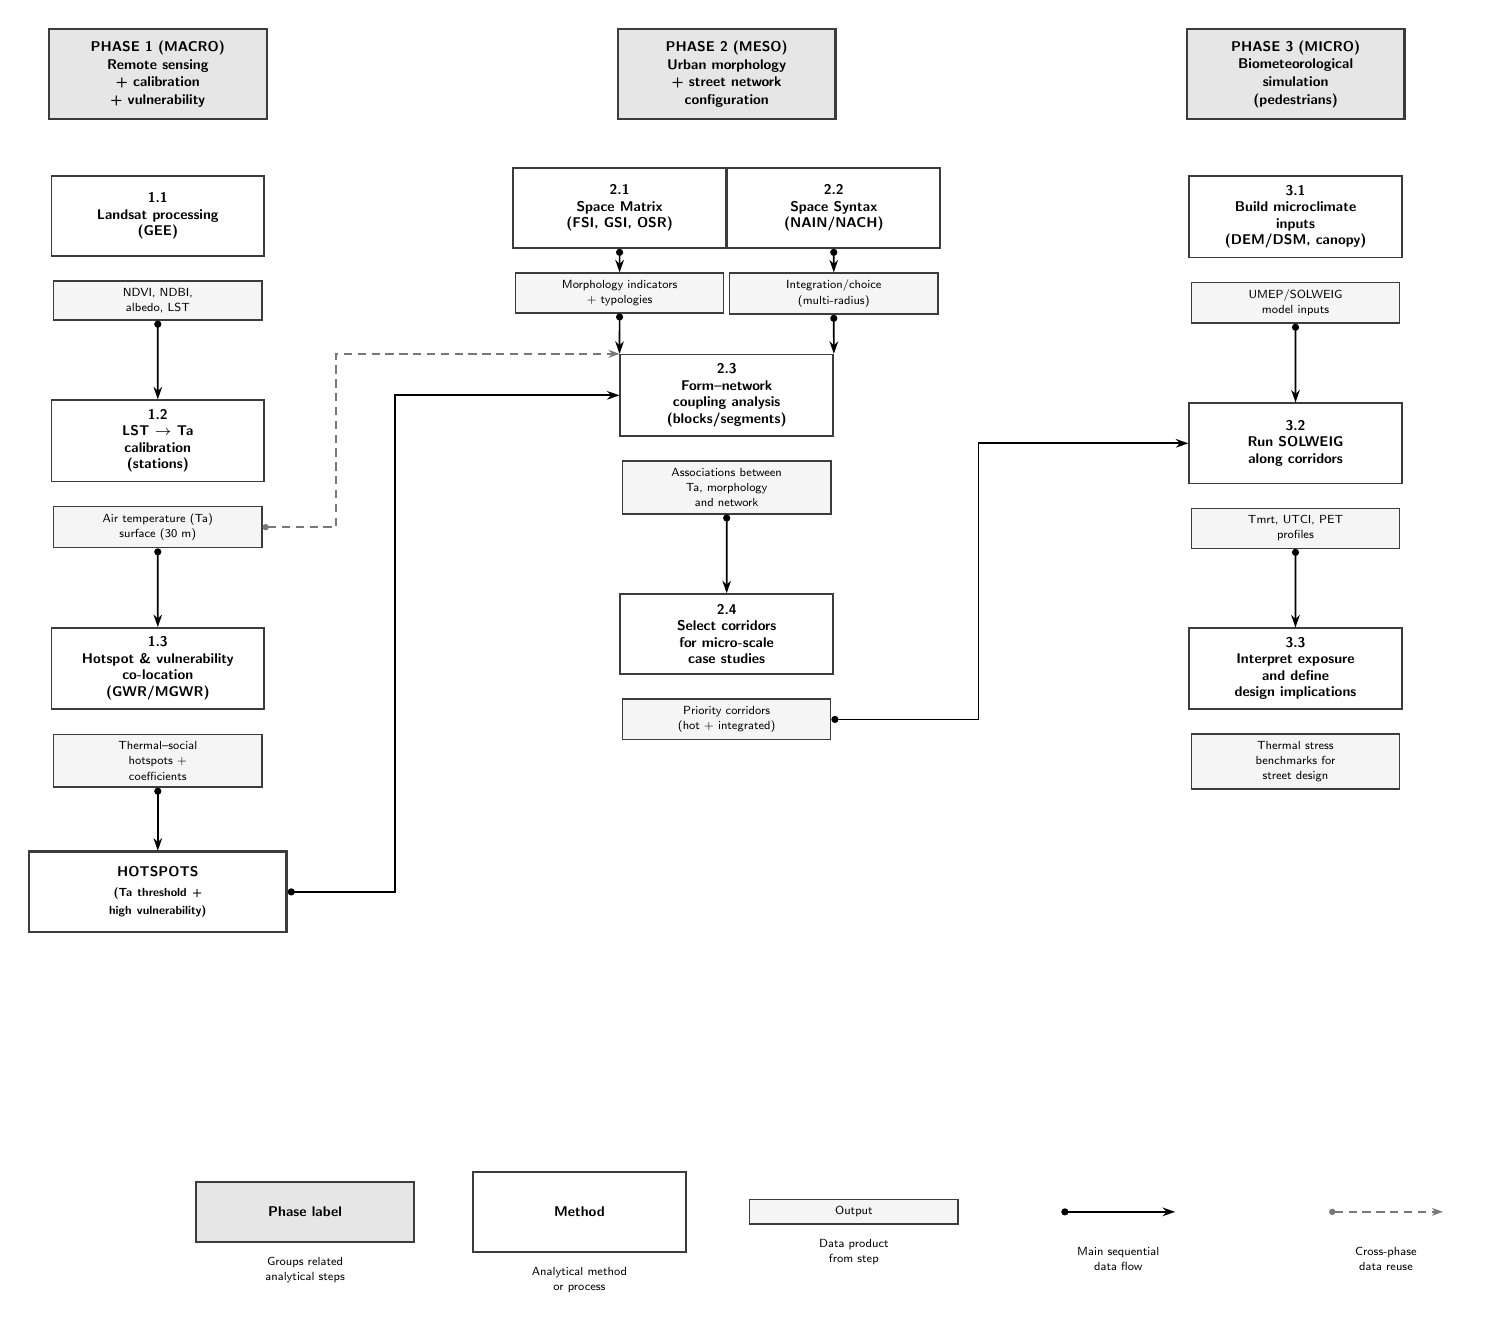
\begin{tikzpicture}[scale=0.85, every node/.style={scale=0.85},
  % Node styles (grayscale)
  stepbox/.style={
    rectangle,
    draw=bordercolor,
    line width=0.6pt,
    fill=stepcolor,
    text width=2.9cm,
    align=center,
    minimum height=1.2cm,
    font=\fontsize{6}{7}\selectfont\bfseries,
    inner sep=4pt
  },
  outputbox/.style={
    rectangle,
    draw=bordercolor,
    line width=0.5pt,
    fill=outputcolor,
    text width=2.9cm,
    align=center,
    font=\fontsize{5.5}{6.5}\selectfont,
    inner sep=3pt
  },
  phaselabel/.style={
    rectangle,
    draw=bordercolor,
    line width=0.8pt,
    fill=phasebg,
    text width=2.9cm,
    align=center,
    font=\fontsize{6.5}{7.5}\selectfont\bfseries,
    inner sep=5pt,
    minimum height=1.1cm
  },
  arrow/.style={
    {Circle[length=0.9mm, fill=arrowcolor]}-{Stealth[length=1.6mm, width=1.1mm]},
    line width=0.6pt,
    draw=arrowcolor
  },
  datareuse/.style={
    {Circle[length=0.8mm, fill=reusecolor]}-{Stealth[length=1.4mm, width=1mm]},
    line width=0.5pt,
    draw=reusecolor,
    densely dashed
  }
]

% ===== PHASE 1 (MACRO) =====
\node[phaselabel] (p1) at (0,10.5) {PHASE 1 (MACRO)\\Remote sensing\\+ calibration\\+ vulnerability};

\node[stepbox, below=0.7cm of p1] (s11) {1.1\\Landsat processing\\(GEE)};
\node[outputbox, below=0.3cm of s11] (o11) {NDVI, NDBI,\\albedo, LST};

\node[stepbox, below=1cm of o11] (s12) {1.2\\LST $\rightarrow$ Ta\\calibration\\(stations)};
\node[outputbox, below=0.3cm of s12] (o12) {Air temperature (Ta)\\surface (30 m)};

\node[stepbox, below=1cm of o12] (s13) {1.3\\Hotspot \& vulnerability\\co-location\\(GWR/MGWR)};
\node[outputbox, below=0.3cm of s13] (o13) {Thermal--social\\hotspots +\\coefficients};

\node[rectangle, draw=bordercolor, line width=0.9pt, fill=white,
      text width=3.5cm, align=center, minimum height=1.2cm,
      font=\fontsize{6.5}{7.5}\selectfont\bfseries,
      inner sep=5pt, below=0.8cm of o13]
      (hotspots) {HOTSPOTS\\[2pt]{\fontsize{5.5}{6.5}\selectfont (Ta threshold +\\high vulnerability)}};
\draw[arrow] (o13.south) -- (hotspots.north);

% ===== PHASE 2 (MESO) =====
\node[phaselabel] (p2) at (8.5,10.5) {PHASE 2 (MESO)\\Urban morphology\\+ street network\\configuration};

\node[stepbox] (s21) at (6.9,8.5) {2.1\\Space Matrix\\(FSI, GSI, OSR)};
\node[outputbox, below=0.3cm of s21] (o21) {Morphology indicators\\+ typologies};

\node[stepbox] (s22) at (10.1,8.5) {2.2\\Space Syntax\\(NAIN/NACH)};
\node[outputbox, below=0.3cm of s22] (o22) {Integration/choice\\(multi-radius)};

\node[stepbox] (s23) at (8.5,5.7) {2.3\\Form--network\\coupling analysis\\(blocks/segments)};
\node[outputbox, below=0.3cm of s23] (o23) {Associations between\\Ta, morphology\\and network};

\node[stepbox, below=1cm of o23] (s24) {2.4\\Select corridors\\for micro-scale\\case studies};
\node[outputbox, below=0.3cm of s24] (o24) {Priority corridors\\(hot + integrated)};

% ===== PHASE 3 (MICRO) =====
\node[phaselabel] (p3) at (17,10.5) {PHASE 3 (MICRO)\\Biometeorological\\simulation\\(pedestrians)};

\node[stepbox, below=0.7cm of p3] (s31) {3.1\\Build microclimate\\inputs\\(DEM/DSM, canopy)};
\node[outputbox, below=0.3cm of s31] (o31) {UMEP/SOLWEIG\\model inputs};

\node[stepbox, below=1cm of o31] (s32) {3.2\\Run SOLWEIG\\along corridors};
\node[outputbox, below=0.3cm of s32] (o32) {Tmrt, UTCI, PET\\profiles};

\node[stepbox, below=1cm of o32] (s33) {3.3\\Interpret exposure\\and define\\design implications};
\node[outputbox, below=0.3cm of s33] (o33) {Thermal stress\\benchmarks for\\street design};

% ===== ARROWS: Main sequential flow =====
\draw[arrow] (o11) -- (s12);
\draw[arrow] (o12) -- (s13);

\draw[arrow] (hotspots.east) -- ++(1.6,0) |- (s23.west);

\draw[arrow] (s21) -- (o21);
\draw[arrow] (s22) -- (o22);
\draw[arrow] (o21.south) -- (s23.north west);
\draw[arrow] (o22.south) -- (s23.north east);
\draw[arrow] (o23) -- (s24);
\draw[arrow] (o24.east) -- ++(2.2,0) |- (s32.west);
\draw[arrow] (o31) -- (s32);
\draw[arrow] (o32) -- (s33);

% ===== Data reuse arrows (cross-phase dependencies) =====
\draw[datareuse] (o12.east) -- ++(1.1,0) |- (s23.north west); % Ta to meso coupling

% ===== VISUAL DICTIONARY =====
\node[phaselabel, minimum width=2.2cm, minimum height=0.9cm] (dict_phase) at (2.2,-6.5) {Phase label};
\node[font=\fontsize{5.5}{6.5}\selectfont, below=0.08cm of dict_phase, text width=2.2cm, align=center] {Groups related\\analytical steps};

\node[stepbox, minimum width=2.2cm] (dict_step) at (6.3,-6.5) {Method};
\node[font=\fontsize{5.5}{6.5}\selectfont, below=0.08cm of dict_step, text width=2.2cm, align=center] {Analytical method\\or process};

\node[outputbox, minimum width=2.2cm] (dict_output) at (10.4,-6.5) {Output};
\node[font=\fontsize{5.5}{6.5}\selectfont, below=0.08cm of dict_output, text width=2.2cm, align=center] {Data product\\from step};

% Arrow examples
\draw[arrow] (13.5,-6.5) -- ++(1.7,0);
\node[font=\fontsize{5.5}{6.5}\selectfont, text width=2.2cm, align=center] at (14.35,-7.2) {Main sequential\\data flow};

\draw[datareuse] (17.5,-6.5) -- ++(1.7,0);
\node[font=\fontsize{5.5}{6.5}\selectfont, text width=2.2cm, align=center] at (18.35,-7.2) {Cross-phase\\data reuse};

\end{tikzpicture}
\caption{Three-scale methodology linking macro screening (thermal--social hotspots), meso characterization (form + network), and micro simulation (pedestrian thermal stress).}
\label{fig:methodology_flow}
\end{figure}
\end{landscape}

\end{document}
